% Created 2024-12-02 一 20:26
% Intended LaTeX compiler: pdflatex
\documentclass[11pt]{article}
\usepackage[utf8]{inputenc}
\usepackage[T1]{fontenc}
\usepackage{graphicx}
\usepackage{grffile}
\usepackage{longtable}
\usepackage{wrapfig}
\usepackage{rotating}
\usepackage[normalem]{ulem}
\usepackage{amsmath}
\usepackage{textcomp}
\usepackage{amssymb}
\usepackage{capt-of}
\usepackage{hyperref}
\author{myu}
\date{\today}
\title{}
\hypersetup{
 pdfauthor={myu},
 pdftitle={},
 pdfkeywords={},
 pdfsubject={},
 pdfcreator={Emacs 27.1 (Org mode 9.3)}, 
 pdflang={English}}
\begin{document}

\tableofcontents

\section{emacs magit,org-mod}
\label{sec:org79667b1}
好久没有更新了,今年看能坚持多久!\\

\subsection{magit使用}
\label{sec:org30fb43e}
\begin{itemize}
\item 此处需要梯子,否则安装很麻烦\\
\end{itemize}
ps: 经过测试,发现如下配置也可以安装,修改源\\

\begin{verbatim}
(setq package-check-signature nil)
(setq package-archives
      '(("gnu"   . "https://elpa.gnu.org/packages/")
	("melpa" . "https://melpa.org/packages/")))
\end{verbatim}

快速唤出方式\\
mysrc + tab 键\\


\begin{itemize}
\item 进入magit界面,按以下键:\\
\end{itemize}
s:add 增加\\
cc:commit 添加注释\\
ctrl c + ctrl c :确认提交\\
P p:push推送到远程\\
帮助信息:ctrl h,m\\

L head , 空格查看,光标不移动;回车查看,光标移动\\

\subsection{magit 常用命令}
\label{sec:orgc858967}
magit-status\\
绑定的命令:ctrl x g\\
s stage;u unstage\\
c , c commit\\
ctrl c,ctrl c 提交\\
推送 push为 P,u 即可完成远程仓库的推送\\

magit-find-file,我们可以比如绑定到C-x m f,它可以指定访问某个分支中某个文件,且是放到一个临时的 buffer,只能说极其好用\\


h 显示帮助命令\\
magit使用的文档,日文版本的,感觉还不错\\
\url{https://joppot.info/posts/f2721fb2-0942-4c4e-90e2-0dbdbb329bce}\\

\subsection{emacs基本使用}
\label{sec:org020c938}
\begin{itemize}
\item 显示文件夹后,在另外窗口打开文件\\
\end{itemize}
ctrl x 4 b\\
ctrl x f ctrl o,焦点不过去\\

\begin{itemize}
\item 复制文本内容ctrl shift @,选择文本内容\\
\end{itemize}
ctrl w 剪切,cmd w 复制\\
ctrl y 粘贴\\

\begin{itemize}
\item 链接\\
\end{itemize}
C-c C-l	编辑链接(此处为小写L)\\
C-c C-o	打开链接(相当有用)\\

具体怎么改你得看org-structure-template-alist的文档(C-h v org-structure-template-alist)\\


\begin{itemize}
\item 滚动屏幕\\
\end{itemize}
滚动另外一个窗口的屏幕向下/向上 ctrl cmd v/ctrl shift cmd v\\

\begin{itemize}
\item rgrep命令搜索文件中的字符串\\
\item find-dired, -iname "\textbf{学习}",搜索所有文件名\\
\item 上面两个命令同时支持中文和 不区分大小写,爽了\\
\end{itemize}

\subsection{dired文件夹模式}
\label{sec:org7d480d4}
\begin{enumerate}
\item 选中文件后,在另外窗口打开,直接 按 o 即可; f 直接在当前缓冲区查看文件\\
\item 焦点不过去,直接查看, ctrl o\\
\item 查看帮助命令,h\\
\item 快速查看blame\\
\item git blame\\
\end{enumerate}
比如我要看当前区域的代码是 who/which commit 提交的。这种都是临时性的需求,因此它是通过特殊 command(C-c M-g b) 以开关的形式操作的(不然看起来太乱了)\\

= 比较文件\\
v 查看文件\\
D 删除文件\\
C 拷贝\\
R 重命名\\
Z 压缩\\
w 复制文件名\\
m 标记\\
u 取消标记\\
\begin{itemize}
\item 新建目录\\
\end{itemize}


C-c *	将本行设置为标题/正文\\

cmd shift \&; 异步执行程序\\
cmd shift !;执行程序,命令行比较少\\

\subsection{emacs windows上使用}
\label{sec:org56ed6b3}
\begin{enumerate}
\item 使用git命令要用eshell方式,其它方式有乱码,没有找到方法如何修改\\
\item eshell中定义alias,快速命令 gs -3 => git log -3\\
\end{enumerate}
\begin{quote}
需要在eshell中执行,alias gs 'git log \$*'\\
每次只执行一次,emacs会自动记忆这个配置,内容保存在.eamcs.d/eshell/alias文件中\\

ps:ctrl c + ctrl , => 快速调用引用 并选择要插入的内容\\
\end{quote}

\subsection{org-mod}
\label{sec:orgb6696d2}
\href{https://www.cnblogs.com/GarfieldEr007/p/5588979.html}{- org教程}\\
\href{https://www.jianshu.com/p/78ef59327e2d}{- org教程2}\\

\href{https://www.cnblogs.com/qlwy/archive/2012/06/15/2551034.html\#sec-4-2}{org教程3}\\
ctrl c,ctrl l ;插入链接\\
ctrl c,' ;插入代码??\\


\subsubsection{org文件导出为html文件}
\label{sec:orgbee1e9e}
\begin{enumerate}
\item org导出html文件\\
\item 编辑完org,要导出ctrl c,ctrl e ,h导出html文件\\
\item 执行sh mv\textsubscript{html2post.sh}\\
\end{enumerate}

\subsubsection{列表和checkbox使用}
\label{sec:org25fb057}
\begin{enumerate}
\item cmd shift ret -- checkbox\\
\begin{itemize}
\item\relax [0/1]\\
\begin{itemize}
\item[{$\square$}] 

\item\relax [100\%]\\
\begin{itemize}
\item[{$\boxtimes$}] 
\end{itemize}
\end{itemize}
\end{itemize}
\item 改变状态方法,ctrl c,ctrl c\\
\item todo ctrl shift ret\\
\end{enumerate}

\subsubsection{其它:}
\label{sec:org1f62735}
\begin{enumerate}
\item cmd 左右,升级降级标题\\
\item 上线两个列表交换位置,cmd shift 上/下\\
\item 循环改变标志符号 ctrl c -\\
\end{enumerate}
ppp4. 标题间跳转\\
\begin{itemize}
\item C-c C-n	下个标题\\
\item C-c C-p	上个标题\\
\item C-c C-f	下个同级的标题\\
\item C-c C-b	上个同级的标题\\
\item C-c C-u	回到上层标题\\
\end{itemize}

\subsubsection{org中到处的文件如何自动把回车放进去}
\label{sec:orgb14d545}
\begin{quote}
在文件开头加上\\
$\backslash$#+OPTIONS: \n:t\\
或者 (setq org-export-preserve-breaks t)\\
\end{quote}
\subsection{标签搜索}
\label{sec:orga21c378}

建立好了tag系统,可以将相关信息收集到一个表中\\

C-c / m 或 C-c $\backslash$ 标准检索, 按照tag进行检索\\
C-c a m 按标签搜索多个文件 需要把文件加入全局agenda\\

\subsection{yasnippet}
\label{sec:org653986d}
支持新建templage\\
ctrl c \& ctrl n\\

\subsection{eww文本浏览器}
\label{sec:org75cb17a}
\begin{enumerate}
\item eww 提示输入浏览网址\\
\item G   重新输入并载入网址\\
\item g   重载\\
\item b/B   添加/显示书签\\
\item \&   外部浏览器打开url\\
\item q   退出\\
\item l/r 后退/前进\\
\item >/< 文件末尾和开头\\
\item w   拷贝文章url\\
\item S   list\\
\item s   switch buffer\\
\item cmd ret 创建新buffer\\
\end{enumerate}

\subsection{vim emacs 快捷键比较}
\label{sec:org23b8337}
\begin{verbatim}
oemacs 与 vim 命令对比(网上摘录)
-----------------------------------------------------------------
exit:                           C-x C-c         :qa /:wq /:xa /:q!
Get back/command mode:          C-g             <esc>
Backward(left):                 C-b             h
Forward(right):                 C-f             l
Next(down):                     C-n             j
Previous(up):                   C-p             k
stArt of line(^):               C-a             0
End of line($):                 C-e             $
mUltiple commands:              C-u nnn cmd     nnn cmd
Multiple commands:              M-digitkey cmd
save File:                      C-x C-s         :w
beginning of buffer:            M-<             1G
end of buffer:                  M->             G
*scroll forward 1 screen*:        C-v             ^F
scroll forward 1/2 screen:                      ^D
scroll forward 1 line:                          ^E
*scroll backward 1 screen*:       M-v             ^B
scroll backward 1/2 screen:                     ^U
scroll backward 1 line:                         ^Y
scroll the other window:        M-C-v
delete under cursor:            C-d             x
delete from cursor to eol:      C-k             D
iSearch forward:                C-s
isearch Reverse:                C-r
Search forward:                 C-s enter       /
search Reverse:                 C-r enter       ?
isearch regexp:                 M-C-s
isearch backward regexp:        M-C-r
search regexp:                  M-C-s enter     /
search backward regexp:         M-C-r enter     ?
Help:                           C-h C-h         :help
Help Apropos:                   C-h a
Help key Bindings:              C-h b           :help [key]
Help Info:                      C-h i
Help Major mode:                C-h m
Help tutorial:                  C-h t           :help howto
Undo:                           C-_             u
Redo:                           C-f             ^R
Mark cursor position:           C-x r SPC       m{a-zA-Z}
eXchange Mark and position:     C-x C-x
goto mark in current file:      C-x r j         '{a-z}
goto mark in any file:                          '{A-Z}
*copy region*:                    M-w             {visual}y
kill region:                    C-w             {visual}d
*Yank and keep buffer*:           C-y
Yank from kill buffer:          M-y             p
convert region to Upper:        C-x C-u         {visual}U
convert region to Lower:        C-x C-l         {visual}u
Insert special char:            C-q octalnum/keystroke
						^V decimal/keystroke
*replace*:                        M-x replace-string      :%s/aaa/bbb/g
replace regexp:                 M-x replace-regexp      :%s/aaa/bbb/g
query replace:                  M-%                     :%s/aaa/bbb/gc
query replace:                  M-x query-replace
query replace regexp:           M-x query-replace-regexp
Open file:                      C-x C-f         :r file
Save file:                      C-x C-s         :w
Save all buffers:               C-x s           :wa
Save as:                        C-x C-w file    :w file
Prompt for buffer:              C-x b
List buffers:                   C-x C-b         :buffers
Toggle read-only:               C-x C-q         :set ro
Prompt and kill buffer:         C-x k
Split vertical:                 C-x 2           :split
Split horizontal:               C-x 3           :vsplit (ver. 6)
Move to other window:           C-x o           ^Wp
Delete this window:             C-x 0           :q
Delete other window(s):         C-x 1           ^Wo
run shell in bg:                M-x compile
kill shell run in bg:           M-x kill-compilation
run make:                                       :make Makefile
check error message:            C-x`            :echo errmsg
run shell and record:           M-x shell       :!script -a tmp
...clean BS, ...                                :!col -b <tmp >record
...save/recall shell record:    C-x C-w record  :r record
run shell:                      M-! sh          :sh
run command:                    M-! cmd         :!cmd
run command and insert:         C-u M-! cmd     :r!cmd
run filter:                     M-| file        {visual}:w file
run filter and insert:          C-u M-| filter  {visual}:!filter
show option                                     :se[t] {option}?
reset option to default                         :se[t] {option}&
reset boolean option                            :se[t] no{option}
toggle boolean option                           :se[t] inv{option}
wrap text at column 72                          :se tw=72
do not wrap                                     :se tw=0
autoindent                                      :se ai
expand tab                                      :se et
————————————————

			    版权声明:本文为博主原创文章,遵循 CC 4.0 BY-SA 版权协议,转载请附上原文出处链接和本声明。
			
原文链接:https://blog.csdn.net/hejinjing_tom_com/article/details/51700911
\end{verbatim}

\subsection{安装自定义的theme}
\label{sec:org05050f6}
github下载文件,zenburn-theme.el\\

(add-to-list 'custom-theme-load-path "\textasciitilde{}/.emacs.d/themes/")\\
(load-theme 'zenburn t)\\

\subsection{如何设计并实现一个百万并发的服务端程序架构}
\label{sec:org22e539c}

\subsection{emacs grep 命令}
\label{sec:org0a04430}

grep --color=auto -nH --null -e "images" -r\\
递归-r\\

\subsection{emacs快速粘贴图片到org文件中}
\label{sec:org17254d1}

html文件中应该是绝对路径\\
/images/11.png\\
**需要手工修改**,此处需要注意\\

脚本要修改,copy的目标路径,html文件的png改为绝对路径\\

显示与不显示图片的快捷键\\
C-c C-x C-v:切换图片的内联显示(toggle inline images)。这个命令可以让你在显示和隐藏图片之间切换。\\

-- \#+ATTR\textsubscript{ORG}: :width 60\%\\
\begin{center}
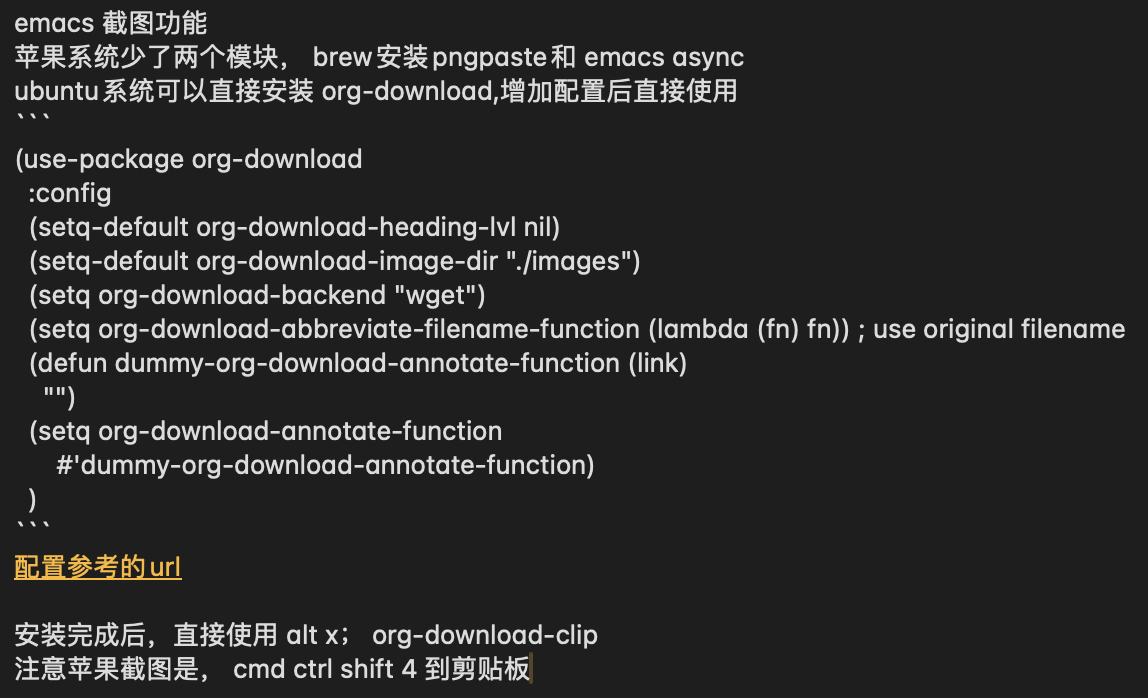
\includegraphics[width=.9\linewidth]{emacs_magit,org-mod/2024-08-14_23-19-36_screenshot.png}
\end{center}

\subsection{如何给shell添加书签}
\label{sec:orgef8c3f3}
emacs shell添加书签未成功,eshell尝试了下可以的\\
eshell是emacs内置shell,完全emacs lisp编写,更集成与emacs环境\\
注意要使用 cd \emph{ssh:myu@192.168.1.13:} 方式打开,没有cd 无法显示正常的文件颜色\\
如下图示例\\

M-x eshell: 启动 Emacs 自己的 shell 实现,它完全用 Emacs Lisp 写成,更加集成 Emacs 功能。\\
M-x term: 这个命令提供了一个更接近传统终端的环境,支持复杂的文本界面,比如那些用于文本编辑器或音乐播放器的界面。\\
M-x ansi-term: 类似于 term,但它更好地支持 ANSI 转义序列,更适合需要运行交互式程序的情况\\
```\\
(defun my-new-eshell ()\\
  "Open a new uniquely named eshell instance."\\
  (interactive)\\
  (let ((eshell-buffer-index (1+ (length (seq-filter (lambda (buf)\\
                                                       (string-prefix-p "\textbf{eshell}" (buffer-name buf)))\\
                                                     (buffer-list))))))\\
    (eshell eshell-buffer-index)))\\

```\\
将这个函数添加到书签中:\\
首先,确保你已经安装并加载了 bookmark 模块。\\
使用 M-x bookmark-set 命令创建一个新书签,当提示你命名书签时,你可以命名为 “New Eshell”。\\
打开书签列表 (M-x bookmark-bmenu-list),找到你刚才创建的书签,然后按 e 来编辑这个书签。\\
将 filename 改为你的 Emacs Lisp 文件位置,并将 handler 设置为 my-new-eshell。\\

\begin{itemize}
\item 打开新的eshell\\
\end{itemize}
通过 C-u M-x eshell 完成。这样做会提示你输入一个缓冲区编号\\


-- \#+ATTR\textsubscript{ORG}: :width 60\%\\
\begin{center}
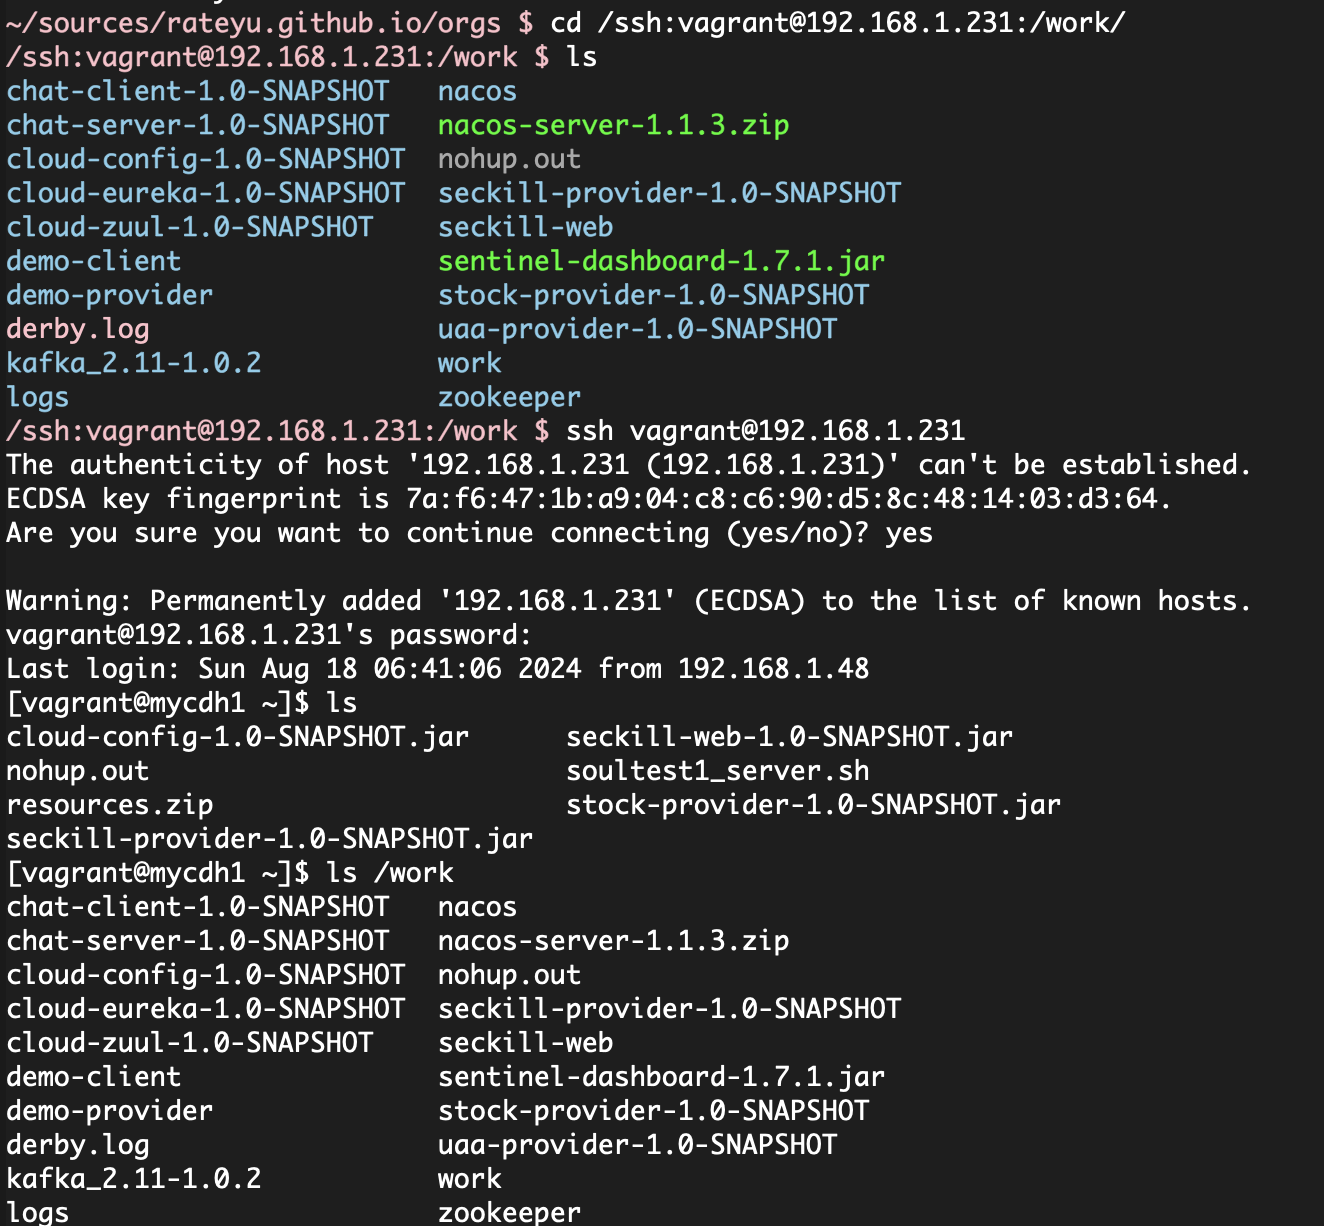
\includegraphics[width=.9\linewidth]{emacs_magit,org-mod/2024-08-18_06-46-51_screenshot.png}
\end{center}

\subsection{eshell 命令行ps -ef | grpe java后,无法显示全命令行参数}
\label{sec:org7062f8e}

```\\
(add-hook 'eshell-mode-hook\\
          (lambda ()\\
            (setq truncate-lines nil)))\\

ps -ef | grep java | less -S\\

```\\

ps: sudo -s 切换到root账号后\\
再ps,可以显示全部命令,并且可以换行\\

\subsection{tcpdump和wirdshark}
\label{sec:orge9a4238}
\begin{verbatim}
tcpdump -n -X -s 0 host 192.168.1.7 -w tt.pcap
- 为命令参数, host为过滤命令
读pcap文件
tcpdump -n -X -r tt.pcap
\end{verbatim}
总结下它们使用命令的联系和区别\\
\end{document}
%%% Local Variables:
%%% mode: latex
%%% TeX-master: t
%%% End:
